% Final Challenge 72 presentation for Overleaf (16:9 Beamer)
\documentclass[aspectratio=169,10pt]{beamer}

\newcommand{\studentname}{S Ayushmaan Patro}
\newcommand{\rollnumber}{CO23BTECH11020}
\newcommand{\institution}{IIT Hyderabad}

% Upload this .tex file beside the existing "figures" folder in Overleaf.
% Required image files:
% figures/workflow.png
% figures/synthetic_validation.png
% figures/benchmark_comparison.png
% figures/external_reference_comparison.png

\usepackage[T1]{fontenc}
\usepackage{lmodern}
\usepackage{graphicx}
\usepackage{booktabs}
\usepackage{array}
\usepackage{xcolor}

\definecolor{navy}{HTML}{17365D}
\definecolor{bluegray}{HTML}{5D7695}
\definecolor{orange}{HTML}{D98C2F}
\definecolor{teal}{HTML}{2F7F7A}
\definecolor{lightbg}{HTML}{F4F7FB}
\definecolor{bodygray}{HTML}{343A40}

\setbeamercolor{normal text}{fg=bodygray,bg=white}
\setbeamercolor{structure}{fg=navy}
\setbeamercolor{frametitle}{fg=white,bg=navy}
\setbeamercolor{title}{fg=navy}
\setbeamercolor{subtitle}{fg=bodygray}
\setbeamercolor{block title}{fg=white,bg=navy}
\setbeamercolor{block body}{fg=bodygray,bg=lightbg}
\setbeamercolor{alerted text}{fg=orange}
\setbeamertemplate{navigation symbols}{}
\setbeamertemplate{itemize item}{\color{orange}\raise0.2ex\hbox{\scriptsize$\blacksquare$}}
\setbeamertemplate{itemize subitem}{\color{teal}\raise0.2ex\hbox{\tiny$\blacktriangleright$}}
\setbeamertemplate{frametitle}{%
  \nointerlineskip
  \begin{beamercolorbox}[wd=\paperwidth,ht=0.82cm,dp=0.23cm,leftskip=0.48cm]{frametitle}
    \usebeamerfont{frametitle}\insertframetitle
  \end{beamercolorbox}}
\setbeamertemplate{footline}{%
  \leavevmode
  \hbox{%
    \begin{beamercolorbox}[wd=.82\paperwidth,ht=2.6ex,dp=1.1ex,leftskip=.45cm]{author in head/foot}
      \color{bluegray}\scriptsize Challenge 72: Hand-Drawn Chemical Structure Recognition
    \end{beamercolorbox}%
    \begin{beamercolorbox}[wd=.18\paperwidth,ht=2.6ex,dp=1.1ex,rightskip=.45cm plus1fil]{date in head/foot}
      \color{bluegray}\scriptsize\hfill\insertframenumber/\inserttotalframenumber
    \end{beamercolorbox}}
  \vskip0pt}

\setbeamerfont{title}{size=\LARGE,series=\bfseries}
\setbeamerfont{subtitle}{size=\large}
\setbeamerfont{frametitle}{size=\Large,series=\bfseries}
\setbeamerfont{normal text}{size=\large}
\setbeamerfont{block title}{size=\normalsize,series=\bfseries}
\setbeamerfont{block body}{size=\normalsize}

\title{Hand-Drawn Chemical Structure Recognition}
\subtitle{Does synthetic drawing-style augmentation improve real-image performance?}
\author{\studentname\ (\rollnumber)}
\institute{\institution\\BT5230 Mini Project -- Challenge 72}
\date{}

\begin{document}

% VIDEO CUE (about 20 seconds): Introduce the topic, your name, and the single
% question tested. Do not discuss results yet.
\begin{frame}[plain]
  \vspace{0.7cm}
  \titlepage
  \vfill
  \begin{center}
    \color{bluegray}\small
    Project-trained MolScribe comparison with an independently labelled DECIMER reference
  \end{center}
\end{frame}

% VIDEO CUE (about 35 seconds): Explain that OCSR converts a chemical drawing
% into a machine-readable molecular string. State why handwriting is harder.
\begin{frame}{Problem and project objective}
  \begin{columns}[T,onlytextwidth]
    \begin{column}{0.52\textwidth}
      \vspace{0.25cm}
      \textbf{Optical chemical structure recognition (OCSR)} converts a molecular depiction into a machine-readable representation such as SMILES.

      \vspace{0.45cm}
      Hand-drawn structures contain uneven bonds, distorted rings, variable spacing, and ambiguous stereochemical marks. These variations create a domain shift from clean computer-rendered images.
    \end{column}
    \begin{column}{0.43\textwidth}
      \begin{block}{Challenge 72 objective}
        Test whether matched synthetic hand-drawn-style augmentation improves recognition of unseen real drawings under student-scale compute.
      \end{block}
      \vspace{0.25cm}
      \textbf{Output:} predicted SMILES, checked for chemical validity and structural agreement.
    \end{column}
  \end{columns}
  \vfill
  {\tiny Source: Rajan et al., Journal of Cheminformatics 16, 2024, article 78.}
\end{frame}

% VIDEO CUE (about 40 seconds): Emphasize that the molecule was split before
% rendering. Both conditions use the same IDs and labels, so augmentation is
% the intended experimental difference.
\begin{frame}{Data and leakage controls}
  \begin{columns}[T,onlytextwidth]
    \begin{column}{0.48\textwidth}
      \textbf{ChEMBL-derived development set}
      \begin{itemize}
        \item 3,758 training molecules
        \item 470 clean validation molecules
        \item 470 held-out synthetic test molecules
        \item Scaffold-separated partitions
      \end{itemize}
    \end{column}
    \begin{column}{0.48\textwidth}
      \textbf{Real benchmark}
      \begin{itemize}
        \item 5,088 DECIMER hand-drawn images
        \item DECIMER test images were not used for training or model selection
        \item Every row retained in the denominator
        \item No retuning after benchmark evaluation
      \end{itemize}
    \end{column}
  \end{columns}
  \vspace{0.35cm}
  \begin{block}{Matched comparison and split provenance}
    Clean and augmented conditions used identical molecule IDs, labels, starting checkpoint, validation images, seed, optimizer settings, and one-epoch duration. The pipeline used the master manifest; separate split CSVs are unchanged inspection exports.
  \end{block}
  \vfill
  {\tiny Dataset: DECIMER Hand-Drawn Molecule Images v1.2, CC BY 4.0.}
\end{frame}

% VIDEO CUE (about 30 seconds): Walk from left to right. The important point is
% that model selection used clean validation data before the real benchmark was examined.
\begin{frame}{Experimental workflow}
  \vspace{0.35cm}
  \begin{center}
    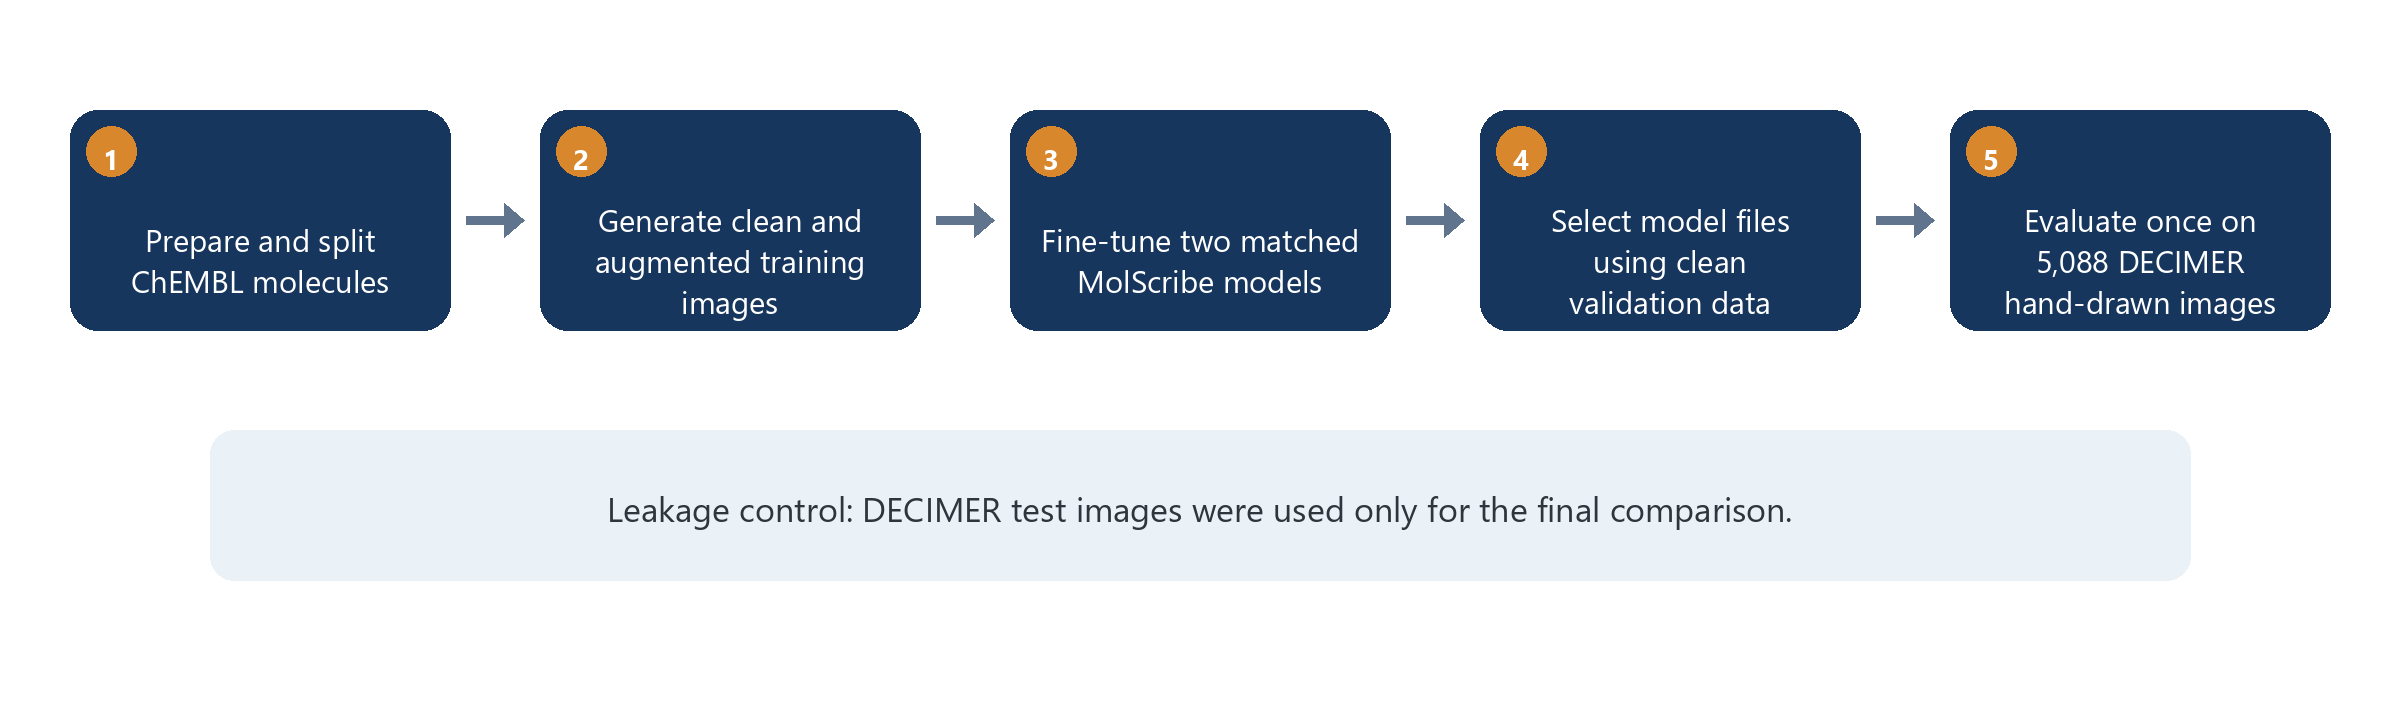
\includegraphics[width=0.98\textwidth]{figures/workflow.png}
  \end{center}
  \vspace{0.15cm}
  \textbf{Independent variable:} training depiction style.\hfill
  \textbf{Primary endpoint:} exact isomeric match on real drawings.
\end{frame}

% VIDEO CUE (about 45 seconds): Briefly describe transfer learning. Explain why
% validity alone is insufficient: a wrong molecule can still be valid SMILES.
\begin{frame}{Model and evaluation metrics}
  \begin{columns}[T,onlytextwidth]
    \begin{column}{0.45\textwidth}
      \textbf{Model}
      \begin{itemize}
        \item Pretrained MolScribe OCSR model
        \item Image encoder and molecular sequence decoder
        \item Clean and augmented one-epoch fine-tuning
        \item Model files selected using clean validation only
      \end{itemize}
    \end{column}
    \begin{column}{0.51\textwidth}
      \textbf{Chemistry-aware metrics}
      \begin{itemize}
        \item Valid SMILES after RDKit sanitization
        \item Exact isomeric match with stereochemistry
        \item Exact non-isomeric match without stereochemistry
        \item Morgan-fingerprint Tanimoto similarity
      \end{itemize}
    \end{column}
  \end{columns}
  \vspace{0.25cm}
  \begin{block}{Conservative scoring}
    Invalid predictions received zero exact-match and zero similarity scores. Paired bootstrap intervals quantified uncertainty between the two checkpoints.
  \end{block}
  \vfill
  {\tiny Checkpoint SHA-256 identifiers and public view-only download links are documented in the submitted README.}
\end{frame}

% VIDEO CUE (about 35 seconds): Say that augmentation looked slightly promising
% on clean synthetic validation. Explain that this justified the held-out test,
% but did not establish performance on real drawings.
\begin{frame}{Synthetic validation showed small gains}
  \begin{columns}[c,onlytextwidth]
    \begin{column}{0.70\textwidth}
      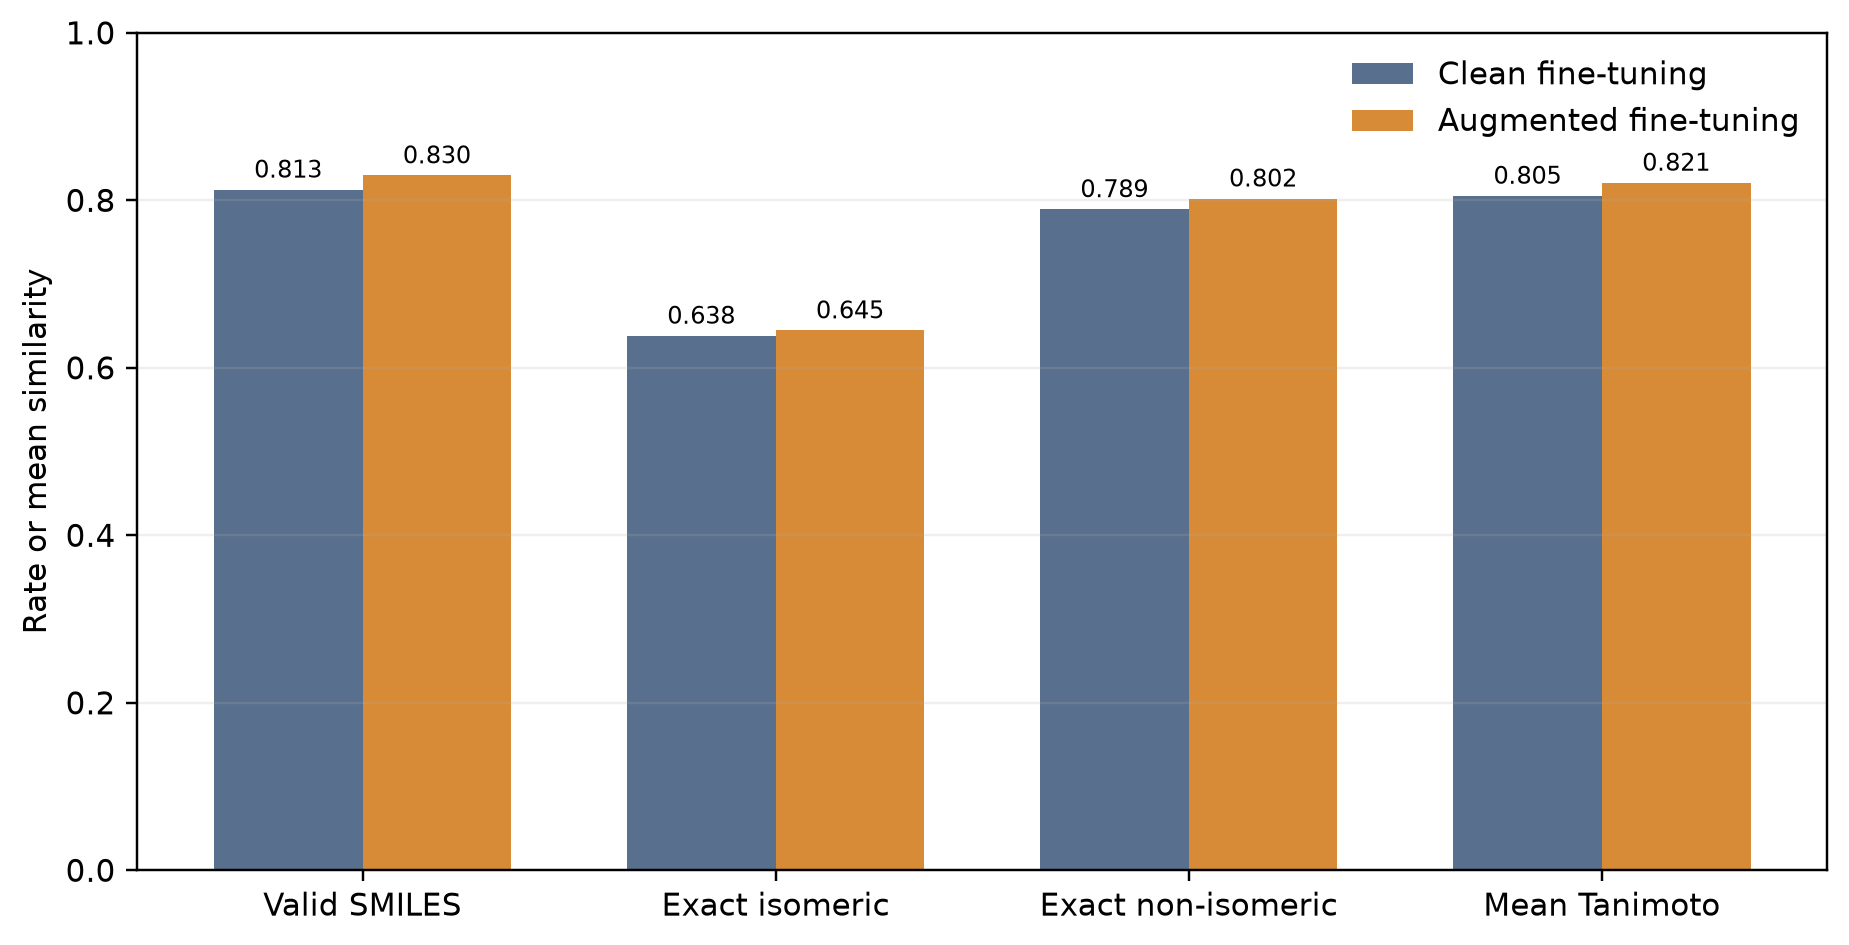
\includegraphics[width=\textwidth]{figures/synthetic_validation.png}
    \end{column}
    \begin{column}{0.27\textwidth}
      \textbf{470 clean images}

      \vspace{0.3cm}
      Exact isomeric:

      63.83\% to 64.47\%

      \vspace{0.3cm}
      Mean Tanimoto:

      0.8054 to 0.8210

      \vspace{0.35cm}
      \alert{This was a feasibility check, not the final real-image result.}
    \end{column}
  \end{columns}
\end{frame}

% VIDEO CUE (about 55 seconds): This is the primary result. Exact accuracy was
% essentially unchanged. Mean Tanimoto decreased slightly with a CI below zero.
% State clearly that the augmentation hypothesis was not supported.
\begin{frame}{Augmentation did not improve the held-out real benchmark}
  \begin{columns}[c,onlytextwidth]
    \begin{column}{0.66\textwidth}
      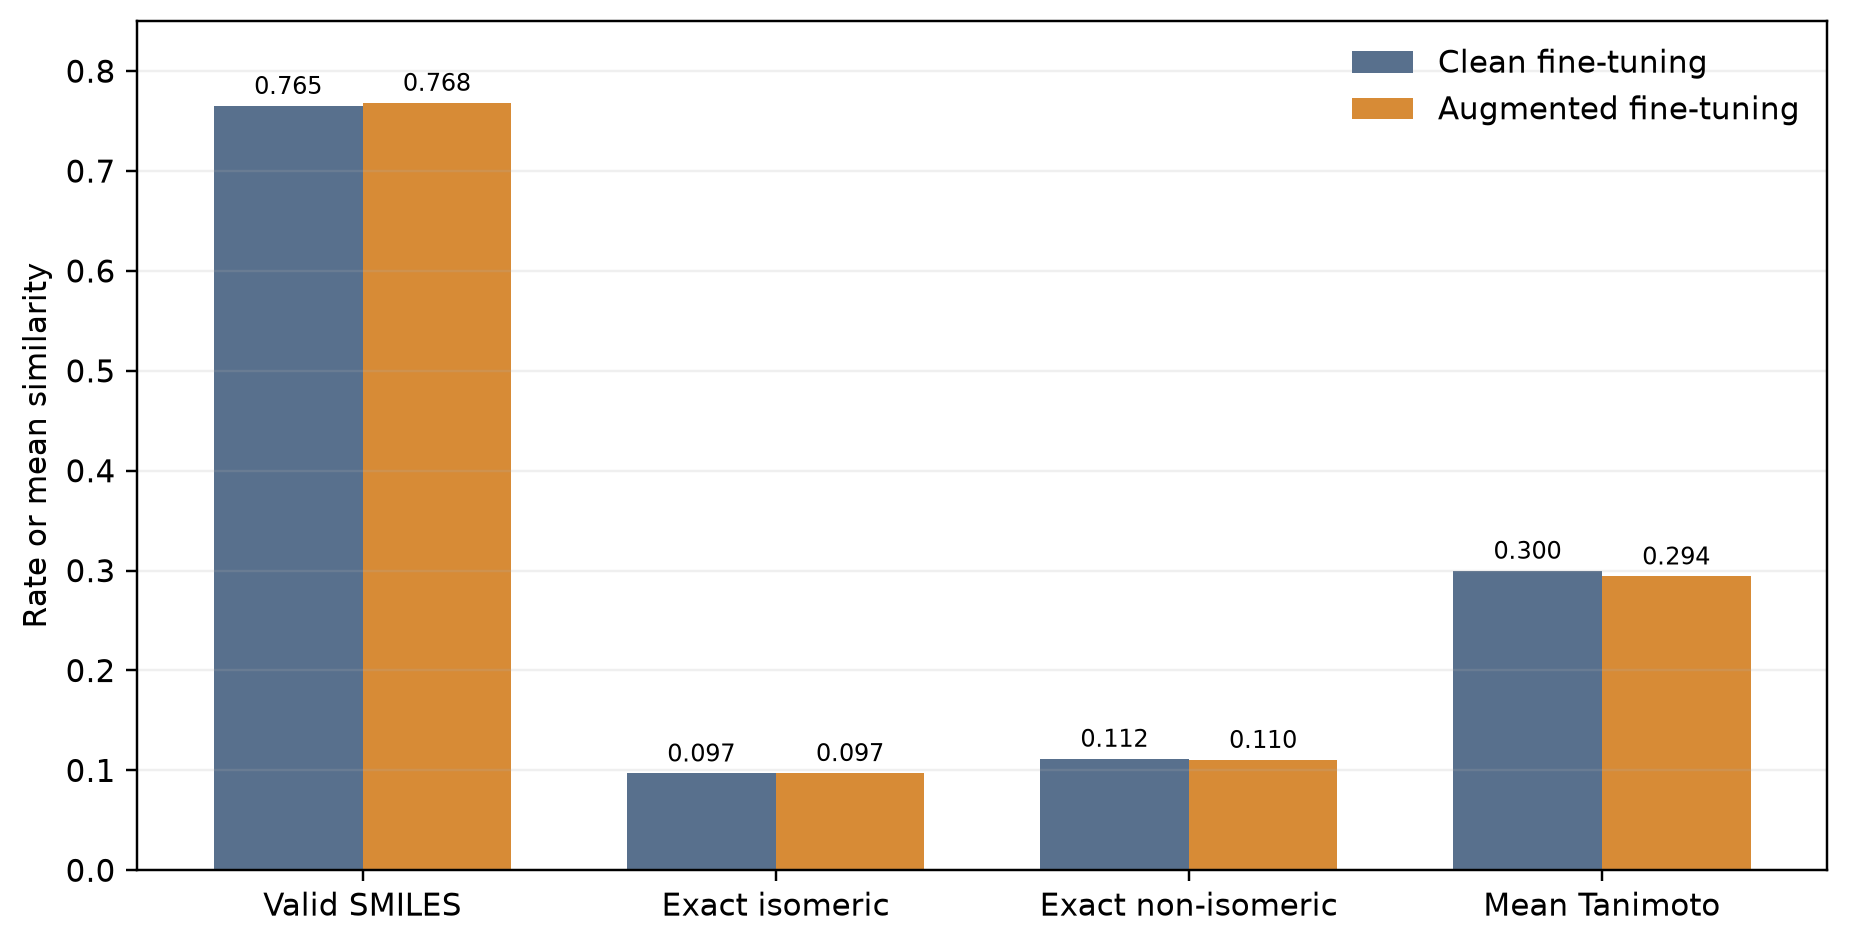
\includegraphics[width=\textwidth]{figures/benchmark_comparison.png}
    \end{column}
    \begin{column}{0.31\textwidth}
      \textbf{All 5,088 images}

      \vspace{0.22cm}
      Exact isomeric:

      9.69\% vs. 9.73\%

      $\Delta=+0.04$ pp

      \vspace{0.25cm}
      Mean Tanimoto:

      0.2998 vs. 0.2941

      $\Delta=-0.0057$

      95\% CI: $[-0.0111,-0.0005]$
    \end{column}
  \end{columns}
  \vspace{0.1cm}
  \alert{Conclusion: the tested augmentation did not improve real-image recognition under this design.}
\end{frame}

% VIDEO CUE (about 50 seconds): Make the ownership distinction explicit. The
% green result is an external pretrained DECIMER model, not a model trained by
% this project. It shows that a domain-specific model can perform much better.
\begin{frame}{External DECIMER reference shows attainable performance}
  \begin{columns}[c,onlytextwidth]
    \begin{column}{0.68\textwidth}
      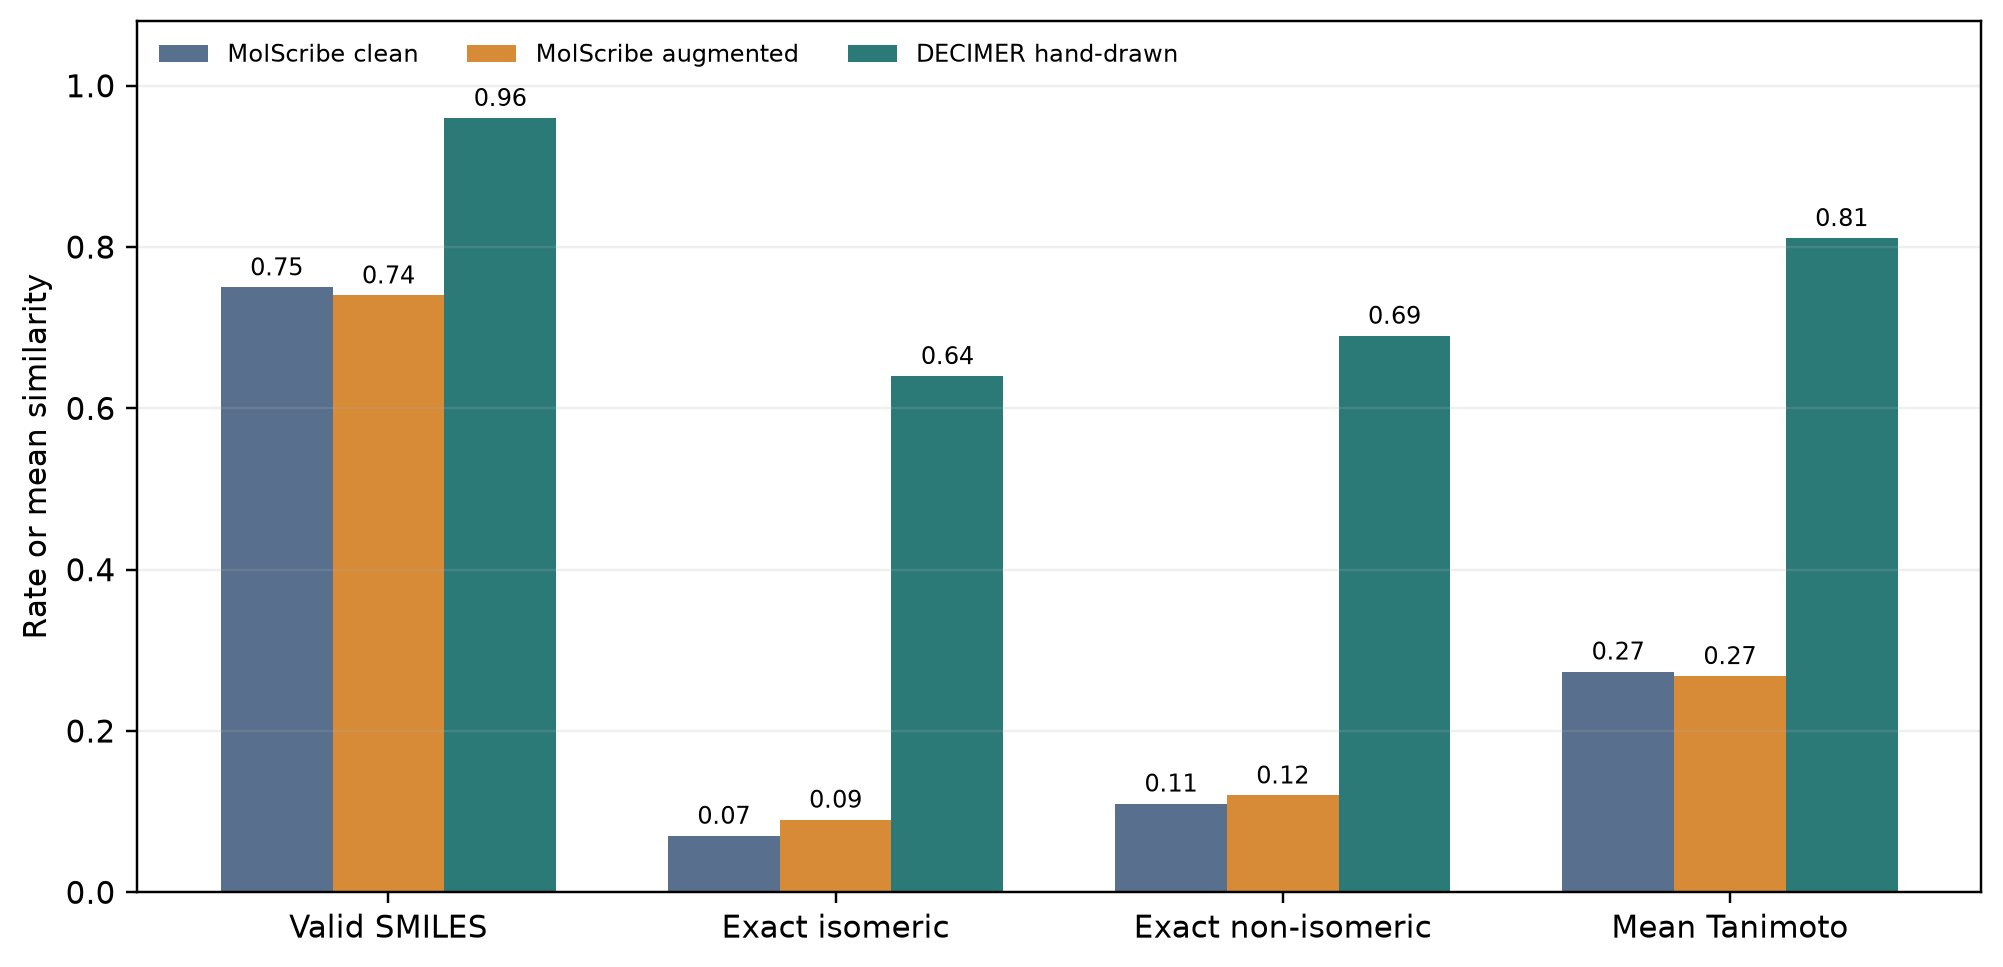
\includegraphics[width=\textwidth]{figures/external_reference_comparison.png}
    \end{column}
    \begin{column}{0.29\textwidth}
      \textbf{Fixed seeded sample}

      100 benchmark images

      \vspace{0.25cm}
      Official DECIMER model:

      64.00\% exact isomeric

      0.8111 mean Tanimoto

      \vspace{0.35cm}
      \alert{External model only. Its weights were not trained or modified in this project.}
    \end{column}
  \end{columns}
  \vfill
  {\tiny DECIMER exact-match Wilson 95\% CI: 54.24\% to 72.73\%. The sample result is not a full-benchmark estimate.}
\end{frame}

% VIDEO CUE (about 55 seconds): Present this slide slowly. Mention the main
% failure pattern, then the safeguards and limitations. Disclose AI assistance
% without claiming that AI independently validated the science.
\begin{frame}{Limitations and research integrity}
  \begin{columns}[T,onlytextwidth]
    \begin{column}{0.48\textwidth}
      \textbf{Observed limitations}
      \begin{itemize}
        \item Accuracy declined for larger, ring-rich, and stereochemically complex structures.
        \item One epoch and 3,758 training molecules limited adaptation.
        \item Synthetic drawing styles did not reproduce the full real-image distribution.
        \item Valid SMILES did not guarantee the correct molecule.
      \end{itemize}
    \end{column}
    \begin{column}{0.48\textwidth}
      \textbf{Integrity safeguards}
      \begin{itemize}
        \item Molecules were split before rendering.
        \item DECIMER test images were used only for the final comparison.
        \item Invalid outputs remained in the denominator.
        \item DECIMER results were labelled as an external reference.
        \item AI tools assisted coding and documentation. The student verified the analysis and remains responsible for all claims.
      \end{itemize}
    \end{column}
  \end{columns}
  \vspace{0.15cm}
  \begin{block}{Responsible use}
    This prototype supports research and digitization workflows. Predictions require expert verification before scientific use.
  \end{block}
\end{frame}

% VIDEO CUE (about 45 seconds): Close with three defensible messages. If asked
% how to improve accuracy, propose better matched augmentation and more
% domain-specific training, evaluated on a newly held-out test set.
\begin{frame}{Conclusions}
  \begin{enumerate}
    \setlength{\itemsep}{0.42cm}
    \item The experiment delivered a leakage-controlled OCSR comparison on all 5,088 real hand-drawn benchmark images.
    \item The tested synthetic augmentation produced small clean-validation gains but did not improve real-image recognition.
    \item The external DECIMER result indicates that larger, domain-specific training can achieve substantially better hand-drawn recognition.
  \end{enumerate}
  \vspace{0.35cm}
  \begin{block}{Next research step}
    Test stronger drawing-style generators and longer transfer schedules using an independent development set, then evaluate once on a newly held-out test set.
  \end{block}
  \vfill
  \begin{center}
    \Large\color{navy}\textbf{Thank you}
  \end{center}
\end{frame}

\end{document}
